\documentclass[UTF8,a4paper,12pt,fontset=windows]{ctexart}

\usepackage{geometry}
\usepackage{graphicx}
\usepackage{float}
\usepackage{booktabs}
\usepackage{array}
\usepackage{longtable}
\usepackage{amsmath}
\usepackage{setspace}
\usepackage{caption}
\usepackage{fancyhdr}
\usepackage[hidelinks]{hyperref}
\usepackage{float}
\usepackage{subcaption}

\geometry{left=2.8cm,right=2.5cm,top=2.8cm,bottom=2.5cm}
\graphicspath{{../图片/}{../图片/程序/}{../图片/视觉软件截图/}}
\setstretch{1.45}
\setlength{\parindent}{2em}
\setlength{\parskip}{0.2em}
\setlength{\headheight}{15pt}
\emergencystretch=2em
\captionsetup{font=small,labelsep=quad}
\pagestyle{fancy}
\fancyhf{}
\fancyhead[C]{《工业机器人工程实践》综合实践报告}
\fancyfoot[C]{\thepage}

\ctexset{
  section = {
    format = \centering\heiti\zihao{3},
    name = {第,章},
    number = \chinese{section},
    aftername = \quad
  },
  subsection = {
    format = \heiti\zihao{4},
    name = {},
    number = \arabic{section}.\arabic{subsection}
  },
  subsubsection = {
    format = \heiti\zihao{-4},
    name = {},
    number = \arabic{section}.\arabic{subsection}.\arabic{subsubsection}
  }
}

\begin{document}

\begin{titlepage}
  \centering
  \vspace*{1.2cm}
  {\zihao{1}\heiti 《工业机器人工程实践》\\[0.5cm]综合实践报告\par}
  \vspace{1.8cm}
  {\zihao{2}\heiti 融合机器视觉与机器人的\\[0.35cm]物品智能分拣系统\par}
  \vfill
  \begin{tabular}{>{\heiti}p{4cm}p{7cm}}
    学生姓名： & 匿名\\[0.35cm]
    学号： & \\[0.35cm]
    班级： & 强基班\\[0.35cm]
    课程名称： & 工业机器人工程实践\\[0.35cm]
    报告日期： & 2026年5月\\
  \end{tabular}
  \vfill
\end{titlepage}

\pagenumbering{Roman}
\section*{摘\quad 要}
\addcontentsline{toc}{section}{摘要}
本实验关注搬运物体、传送物体以及智能分拣，整个系统由直角坐标机器人、直线伺服机器人、Delta机器人、机器视觉检测系统还有PLC控制系统组成。直角坐标机器人从左侧初始区域抓取物料放到托盘上，直线伺服机器人把托盘运输到右侧Delta机器人的分拣处，Delta机器人则依据目标区域机器视觉检测结果进行分类摆放。直角和Delat机器人的两个视觉系统分别完成初始、分拣、目标位置以及物料颜色、形状信息的检测，并且受PLC信号触发拍照以及数据传输。PLC程序可分为一下几个部分：使能复位、与视觉通信、抓取放置物品、托盘传送以及Delta分拣，于是各执行机构可按PLC程序规定的顺序协同工作。调试过程中主要遇到了PLC写入异常、VisionMaster触发逻辑不匹配以及Delta机器人边缘区域误差较大这几个较大的问题，并在报告里对本组采用的解决方法进行了汇报和分析。在报告最后对整个实验，包括硬件与软件实现、视觉标定、通信联动、安装调试和误差改进等等部分进行了总结。

\noindent\textbf{关键词：}直角坐标机器人；Delta机器人；视觉分拣

\clearpage
\tableofcontents
\clearpage
\pagenumbering{arabic}

\section{概述}

工业机器人分拣系统是典型的机、电、控、视一体化应用场景。它不仅要求单个执行机构能够完成稳定的定位运动，还要求多个机构能够按照统一节拍进行协同工作。在本实验中，物品最初被无序摆放在左侧初始区域，机器视觉系统需要先识别它们的几何中心，再驱动机器人进行抓取传送以及分类摆放。整个过程当中，视觉系统主要提供位置信息，PLC程序则承担机器人运动调度，而两个机器人机构负责实际的物品搬运。

本项目选用直角坐标机器人承担开始的搬运任务，选用直线伺服机器人承担中间传送任务，选用Delta机器人承担最后的分拣任务。直角坐标机器人具有结构直观、定位关系清晰的特性，适宜用于物品拾取；直线伺服机器人可以稳定传送托盘上的物品，Delta机器人具有末端移动速度快、工作空间较大的特点因而适合平面分拣，适用于对目标区域内的物料进行快速放置。

和单一机器人运动控制相比，本系统的难点集中在以下三个方面。第一，视觉坐标与机器人坐标之间需要完成标定转换，否则识别结果无法用于抓取。第二，PLC、视觉软件和多个执行机构之间需要建立稳定的通信逻辑，避免出现误触发、重复触发等问题。第三，Delta机器人在工作空间边缘区域存在一定非线性误差，需要结合实际调试结果进行补偿。围绕以上这些问题，本报告对系统设计与具体实现过程进行整理，并详细说明PLC程序、视觉软件配置以及调试问题处理过程。

\section{工程实践任务及要求}

\subsection{设计任务}

根据题目，本实验可分为以下几个阶段：视觉系统检测不同颜色物品的位置；直角坐标机器人依据检测出的位置移动并在适当时候给电磁铁通电来抓取物品，然后把物品放置到伺服直线传送托盘上；伺服直线机器人把托盘移动至Delta机器人工作区域；Delta机器人的视觉系统对托盘或目标区域进行拍照检测；Delta机器人依据视觉检测出的位置进行物品的抓取与摆放。上述阶段机器人的动作和视觉流程由PLC程序统一调度，按序执行。

\begin{figure}[H]
  \centering
  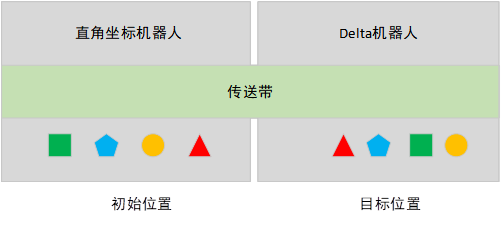
\includegraphics[width=0.72\textwidth]{题目示意图.png}
  \caption{系统设计任务示意图}
  \label{fig:task}
\end{figure}

\subsection{设计要求}

根据《工业机器人工程实践》综合设计内容及考核要求，本系统需要由直线伺服模型、直角坐标机器人模型、Delta机器人模型和视觉检测系统四部分组成，并且完成个体运动控制和总体协同控制。系统应具备显示、急停保护和初始化复位功能，视觉检测功能也需要受PLC信号控制。

设计要求可以进一步分解为以下几个方面。其一，直角坐标机器人需要完成对初始区域物品的定位和抓取，并且能够根据视觉坐标对抓取点进行调整。其二，伺服直线模组需要完成指定位置之间的托盘传送，使物品能够稳定进入Delta机器人分拣区域。其三，Delta机器人需要根据目标视觉系统提供的物品类别和坐标信息，把物品摆放到对应目标位置。其四，两个视觉系统需要分别检测物品初始位置、目标位置以及颜色、形状等分类信息。其五，视觉系统与机器人控制系统之间需要实现双向通信，机器人能够根据视觉数据执行动作，视觉拍照也能够由PLC信号触发。其六，整个抓取、传送和分拣流程需要由启动开关启动，并在运行过程中保持自动化顺序控制。

\section{理论设计}

\subsection{系统设计}

整个系统可分为四个层级。最上层负责整体控制的是PLC程序，管理视觉通信变量读写和机器人运动指令的调用。第二层则是VisionMaster视觉系统，关注并检测直角坐标机器人抓取区域和Delta机器人分拣区域的物品。第三层是由直角坐标机器人、直线伺服机器人、Delta机器人和电磁铁这些个执行机构组成的。最后一层则包括启动、复位、急停等部分。

PLC程序并不是简单地同时驱动多个机构，而是以“状态转移”的方式安排动作顺序。系统启动后，先进行使能和复位，使各轴处于可执行运动指令的状态；随后触发初始视觉拍照，并等待视觉结果稳定返回；PLC根据视觉返回坐标驱动直角坐标机器人运动到抓取点；抓取完成后，直角坐标机器人把物品放到传送托盘上；直线伺服机器人把托盘送到分拣工位；Delta机器人先移开以避免遮挡相机，视觉系统再次拍照；最后Delta机器人根据目标区域识别结果完成物料抓取和分类放置。系统工作流程如表\ref{tab:workflow}所示。

\begin{longtable}{p{1.5cm}p{4.2cm}p{8.1cm}}
  \caption{系统工作流程设计}\label{tab:workflow}\\
  \toprule
  序号 & 流程环节 & 主要内容\\
  \midrule
  1 & 初始化 & PLC完成轴使能、错误复位、机构回到初始位置。\\
  2 & 初始视觉检测 & 直角机器人侧视觉系统检测物品初始坐标、颜色和形状。\\
  3 & 前端抓取 & 直角坐标机器人按照视觉检测给出的坐标移动，使用电磁铁抓取物品并完成放置。\\
  4 & 伺服传送 & 直线伺服模组把承载物品的托盘送到Delta机器人区域。\\
  5 & 分拣视觉检测 & Delta机器人移开相机视野，该侧视觉系统获取分类和位置数据。\\
  6 & Delta分拣 & Delta机器人依据视觉系统识别的结果抓取物品，并摆放到指定位置。\\
  7 & 复位 & 单次动作完成或出现错误后，点按复位按钮系统错误复位并进入待命状态。\\
  \bottomrule
\end{longtable}

\subsection{机器人运动学分析}

本实验采用的三轴直角坐标机器人由三条相互垂直的直线轴组成，执行机构无法旋转，因此末端位姿可以直接由各轴位移表示。以机器人基坐标系建立坐标，末端位置可表示为
\[
P = (x, y, z)
\]
其中$x$、$y$、$z$分别对应三个直线轴的位置。因此视觉识别出的目标点经过标定后只需做简单的线性矫正就能直接作为直角机器人运动控制指令中的目标位置。为了避免末端与物品或托盘碰撞，在抓取时我们进行了三角形的路径规划，从抓取高度抬升到安全高度，进行平面内的移动，然后再下降到放下高度。

Delta机器人属于并联机构，末端平台的位置由多组连杆共同约束。相较于直角坐标机器人，它的运动学关系更加复杂。本实验中Delta机器人侧并不过分关注在程序里进行完整Delta机器人的运动学模型的推导与应用，而是通过标定把视觉像素坐标转换为物品分拣平面的坐标，并在控制程序中调用Delta机器人相关的运动指令执行末端定位。 Delta机器人的配置界面如图\ref{fig:delta-config}所示，该配置为后续Delta机器人根据末端坐标解算关节角度实现物品抓取提供了坚实的基础。

\begin{figure}[H]
  \centering
  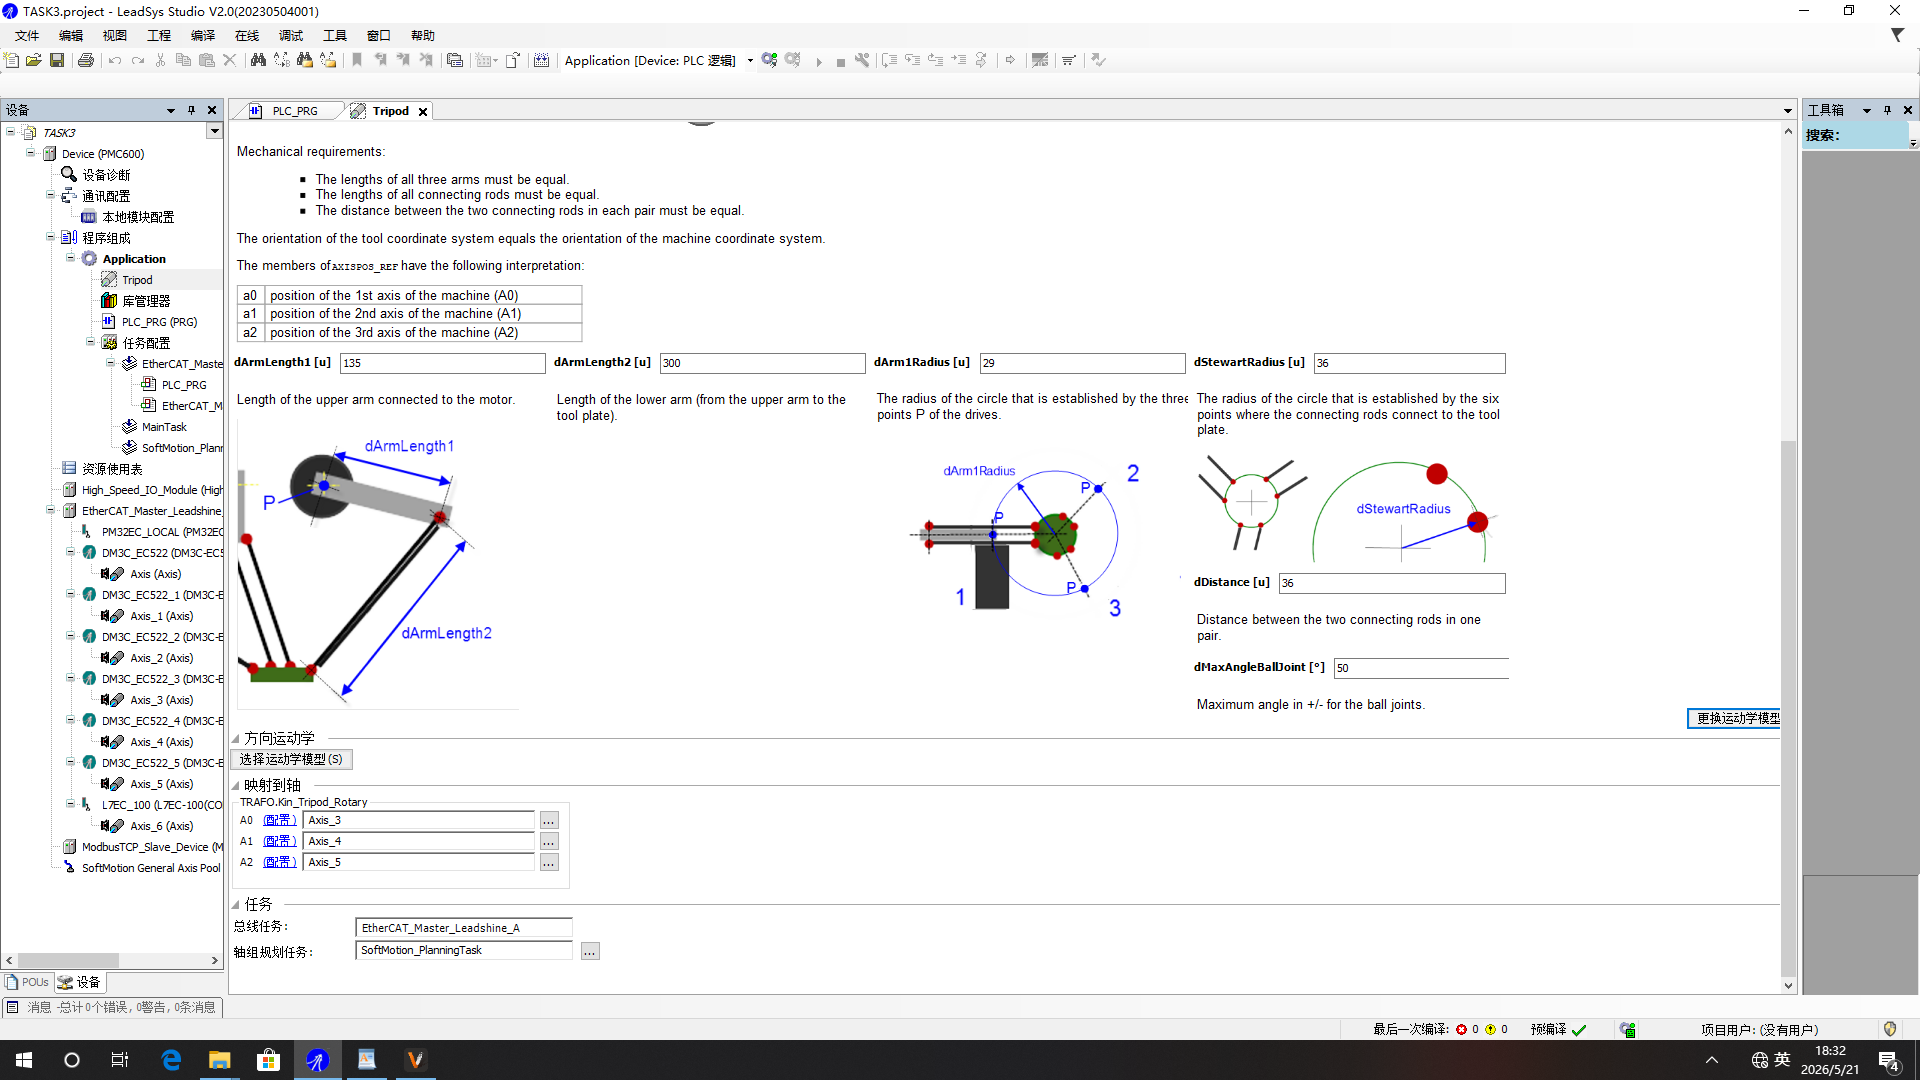
\includegraphics[width=0.88\textwidth]{delta机器人配置图.png}
  \caption{Delta机器人配置界面}
  \label{fig:delta-config}
\end{figure}

对于视觉坐标转换，标定的基本目标是建立像素坐标$(u,v)$与机器人坐标$(x,y)$之间的对应关系。最开始使用的是软件里自带的标定版进行标定，如\ref{fig:vm-calib}所示，但是注意到Delta机器人在中心区域抓取精度高，和初步方案曾采用二维仿射模型：
\[
\begin{bmatrix}
x\\
y
\end{bmatrix}
=
\begin{bmatrix}
a_{11} & a_{12}\\
a_{21} & a_{22}
\end{bmatrix}
\begin{bmatrix}
u\\
v
\end{bmatrix}
+
\begin{bmatrix}
b_1\\
b_2
\end{bmatrix}
\label{biaoding}
\]
实际拟合得到的Delta侧坐标换算关系为：
\[
\begin{aligned}
DelatX &= -0.253990 \cdot PixelX - 0.009306 \cdot PixelY + 57.632354\\
DelatY &= -0.007413 \cdot PixelX - 0.276420 \cdot PixelY + 63.088810
\end{aligned}
\]
我们预计该模型可以修正平移、旋转、比例和剪切等线性误差，但实际对于Delta机器人工作空间边缘的非线性误差改善有限。因此后续调试中结合实际误差分布引入了经验补偿，使边缘区域放置精度得到提升。

\subsection{轨迹规划}

轨迹规划，安全优先。直角坐标机器人抓取物料时，先在吸附高度给电磁铁通电来抓取物品，然后抬升至安全高度并在此平面移动到托盘指定位置上方，然后下降至放下高度并断电放下物品。

直线伺服机器人的轨迹规划则相对简单，主要是在初始工位和分拣工位之间进行位置定位控制。为了避免托盘到位前Delta机器人提前动作，PLC程序里有设置先到位信号后视觉触发的顺序。只有当伺服直线机器人完成传送并且目标区域满足拍照条件后，视觉拍照识别流程才会被触发。

Delta机器人分拣轨迹同样采用安全高度过渡。Delta机器人连杆可能遮挡相机视野，所以程序中就设置了“Delta移开拍照”的动作，在物品搭乘托盘来到分拣区域之前把Delta机器人移出相机视野，确保视觉系统能够拍到完整的物品。拍照完成后，Delta机器人会再次回到分拣区域，根据刚刚移开时候的视觉识别结果进行物品的抓取和放置。对于最终放下物品阶段，我们在实验中额外降低了速度和加速度，使物品在接近目标位置时运动更加平稳，有效的减小了惯性和机构误差带来的偏差。

\section{系统集成与实现}

\subsection{硬件连接与配置}

PLC通过运动控制指令驱动直角坐标、直线伺服和Delta这三大机器人，并且利用输出线圈（\%QX3.0和\%QX3.2）输出电压来分别控制直角机器人侧和Delta机器人侧的电磁铁。视觉系统与PLC之间进行整型变量通信，视觉软件根据PLC发送的数据触发上升沿事件，事件触发启动拍照检测全流程，并把识别到的位置、颜色和形状信息反馈给PLC。

PMC600运动控制指令手册中说明，PMC控制器的运动控制指令以PLCopen运动控制功能块为基础，常用指令包括轴使能、错误复位和绝对定位运动等。本实验中，轴上电和运行准备阶段对应MC\_Power类使能逻辑；异常清除和重新运行准备对应MC\_Reset类复位逻辑；各机构移动到指定抓取点、等待点和放置点时，则主要依靠绝对定位运动MoveAbsolute类指令完成。这样的功能块组织方式使PLC程序能够按照明确状态调用运动功能，也便于在调试中观察每个动作环节的完成状态。

在实验中，我们注意到直角坐标和Delta机器人需要分别设定安全、抓取和放置这三大高度。伺服直线机器人需要额外设定起点、终点、正确的回零方式，还要注意运行速度设置合理，避免运行过程里物品在托盘上抖动剧烈。电磁铁控制需要和机器人运动状态准确配合，正确选择上升沿或高电平信号，避免在错误的时机吸附导致精度下降或者抓取放下失败。视觉系统则需要完成正确且精准的相机标定、识别流程配置和通信变量绑定。

\subsection{软件实现}

\subsubsection{PLC程序结构}

图\ref{fig:plc-enable}展示了轴组使能与复位部分程序，系统只有在7个电机被使能和复位后，才会进入后续自动流程。
视觉通信部分如图\ref{fig:plc-vision-comm}所示。PLC与VisionMaster之间的数据传输就依靠这几行代码。
直角坐标机器人侧的电磁铁控制如图\ref{fig:plc-cart-mag}所示。该部分用于在末端移动到物品抓取点时给电磁铁通电来抓取，并在移动到托盘放置点时断电释放。电磁铁动作必须与Z轴下降和抬升动作配合，避免出现抓取失败、释放过早等问题。Delta机器人侧电磁铁控制如图\ref{fig:plc-delta-mag}所示，与直角机器人侧逻辑相似所以就不再赘述。

\begin{figure}[H]
	\centering
	
	\begin{subfigure}[t]{0.49\textwidth}
		\centering
		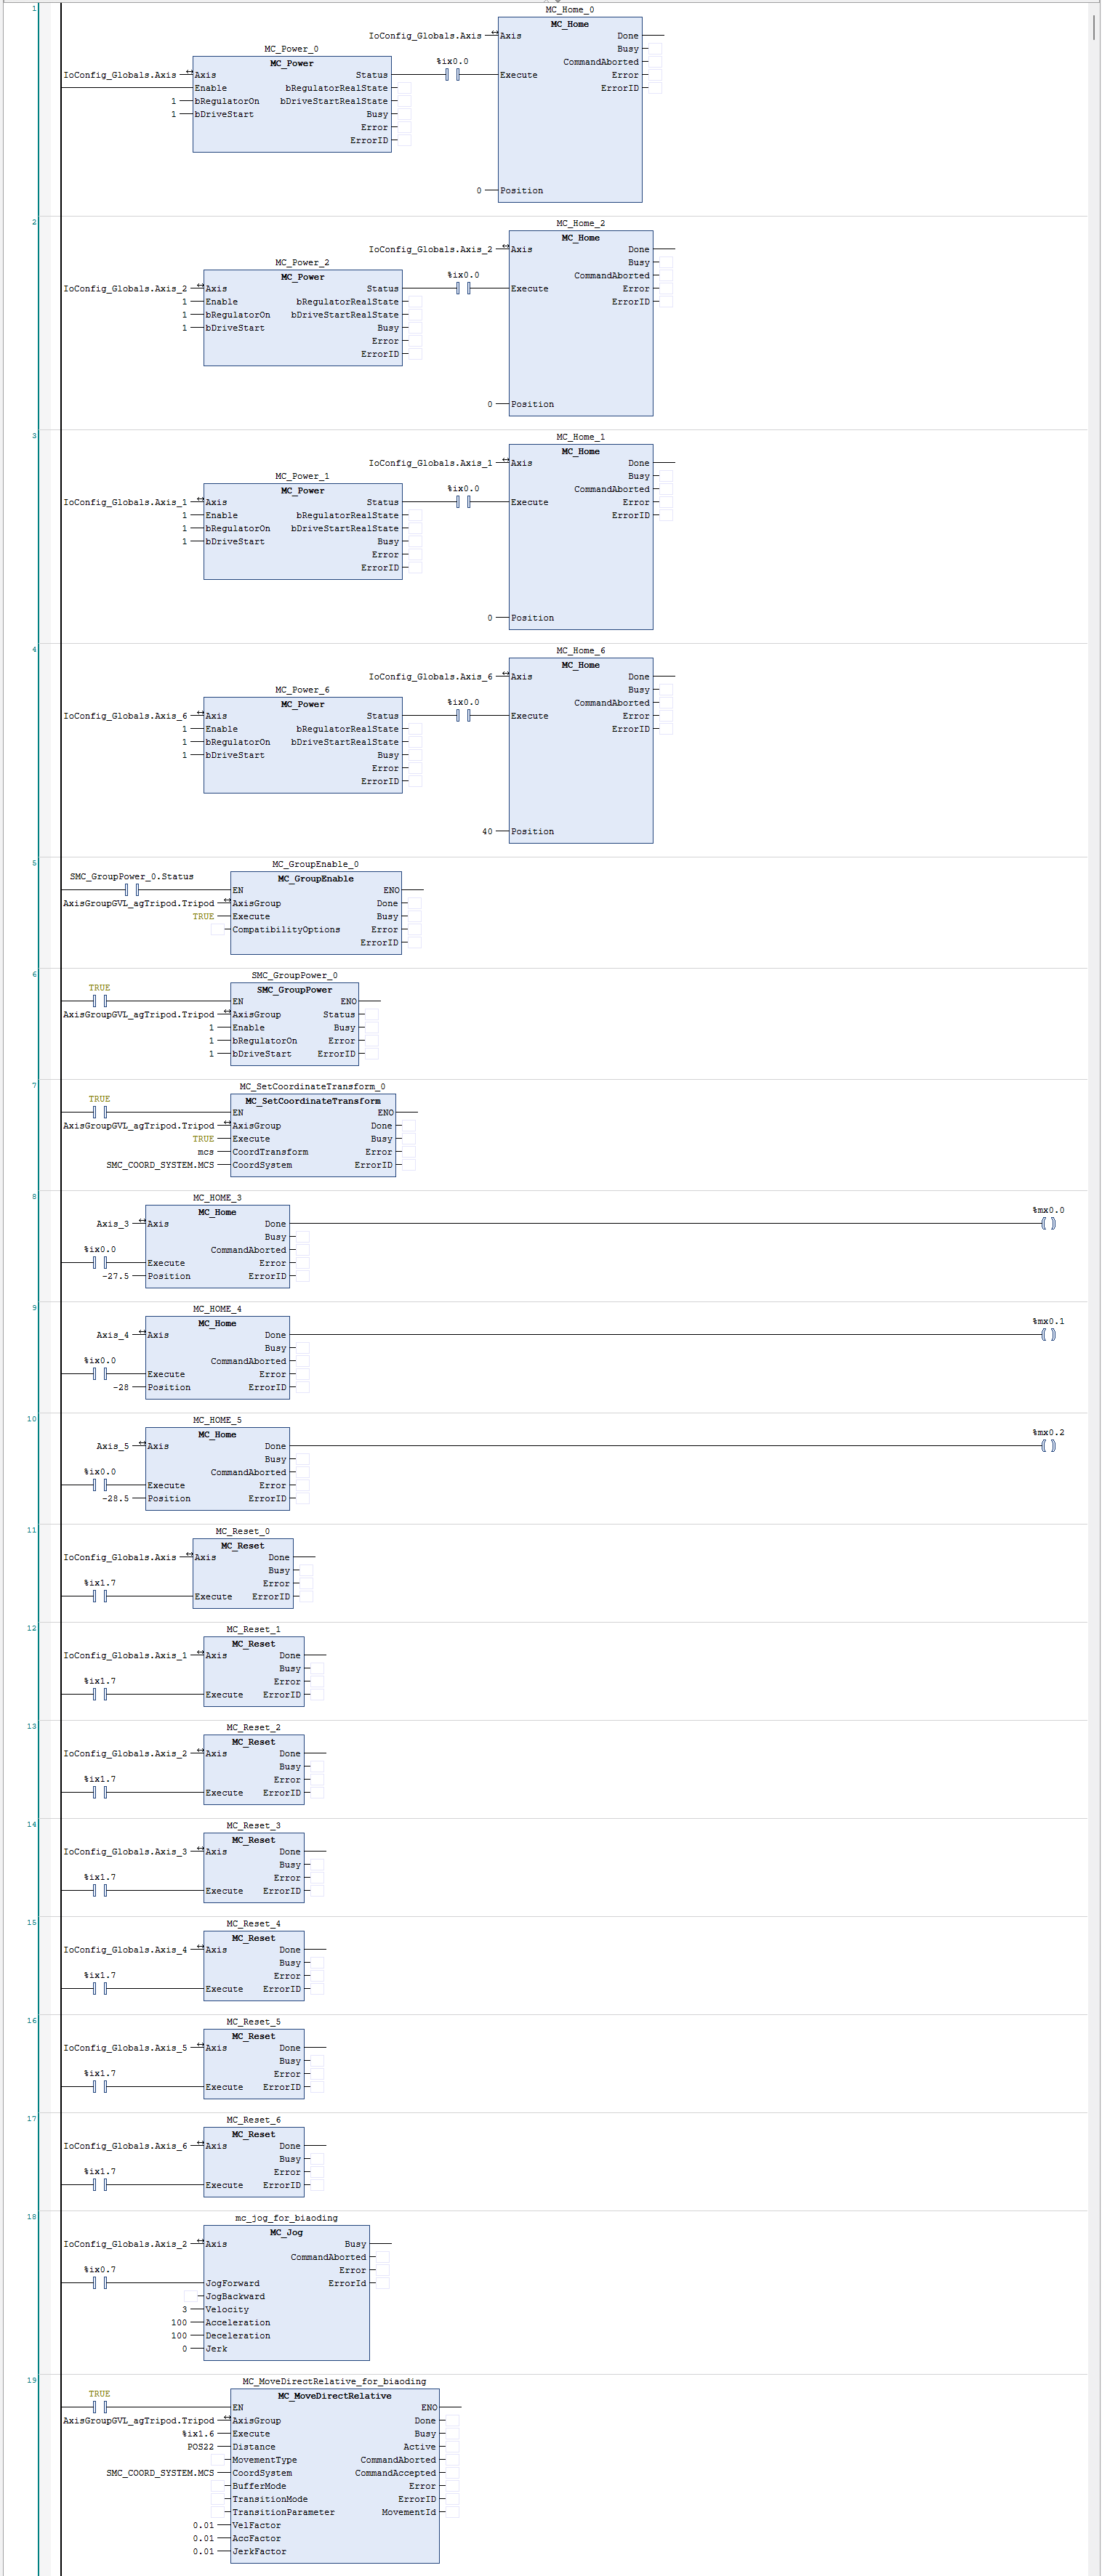
\includegraphics[width=\linewidth,height=0.42\textheight,keepaspectratio]{1准备使能与复位.png}
		\caption{准备使能与复位}
		\label{fig:plc-enable}
	\end{subfigure}
	\hfill
	\begin{subfigure}[t]{0.49\textwidth}
		\centering
		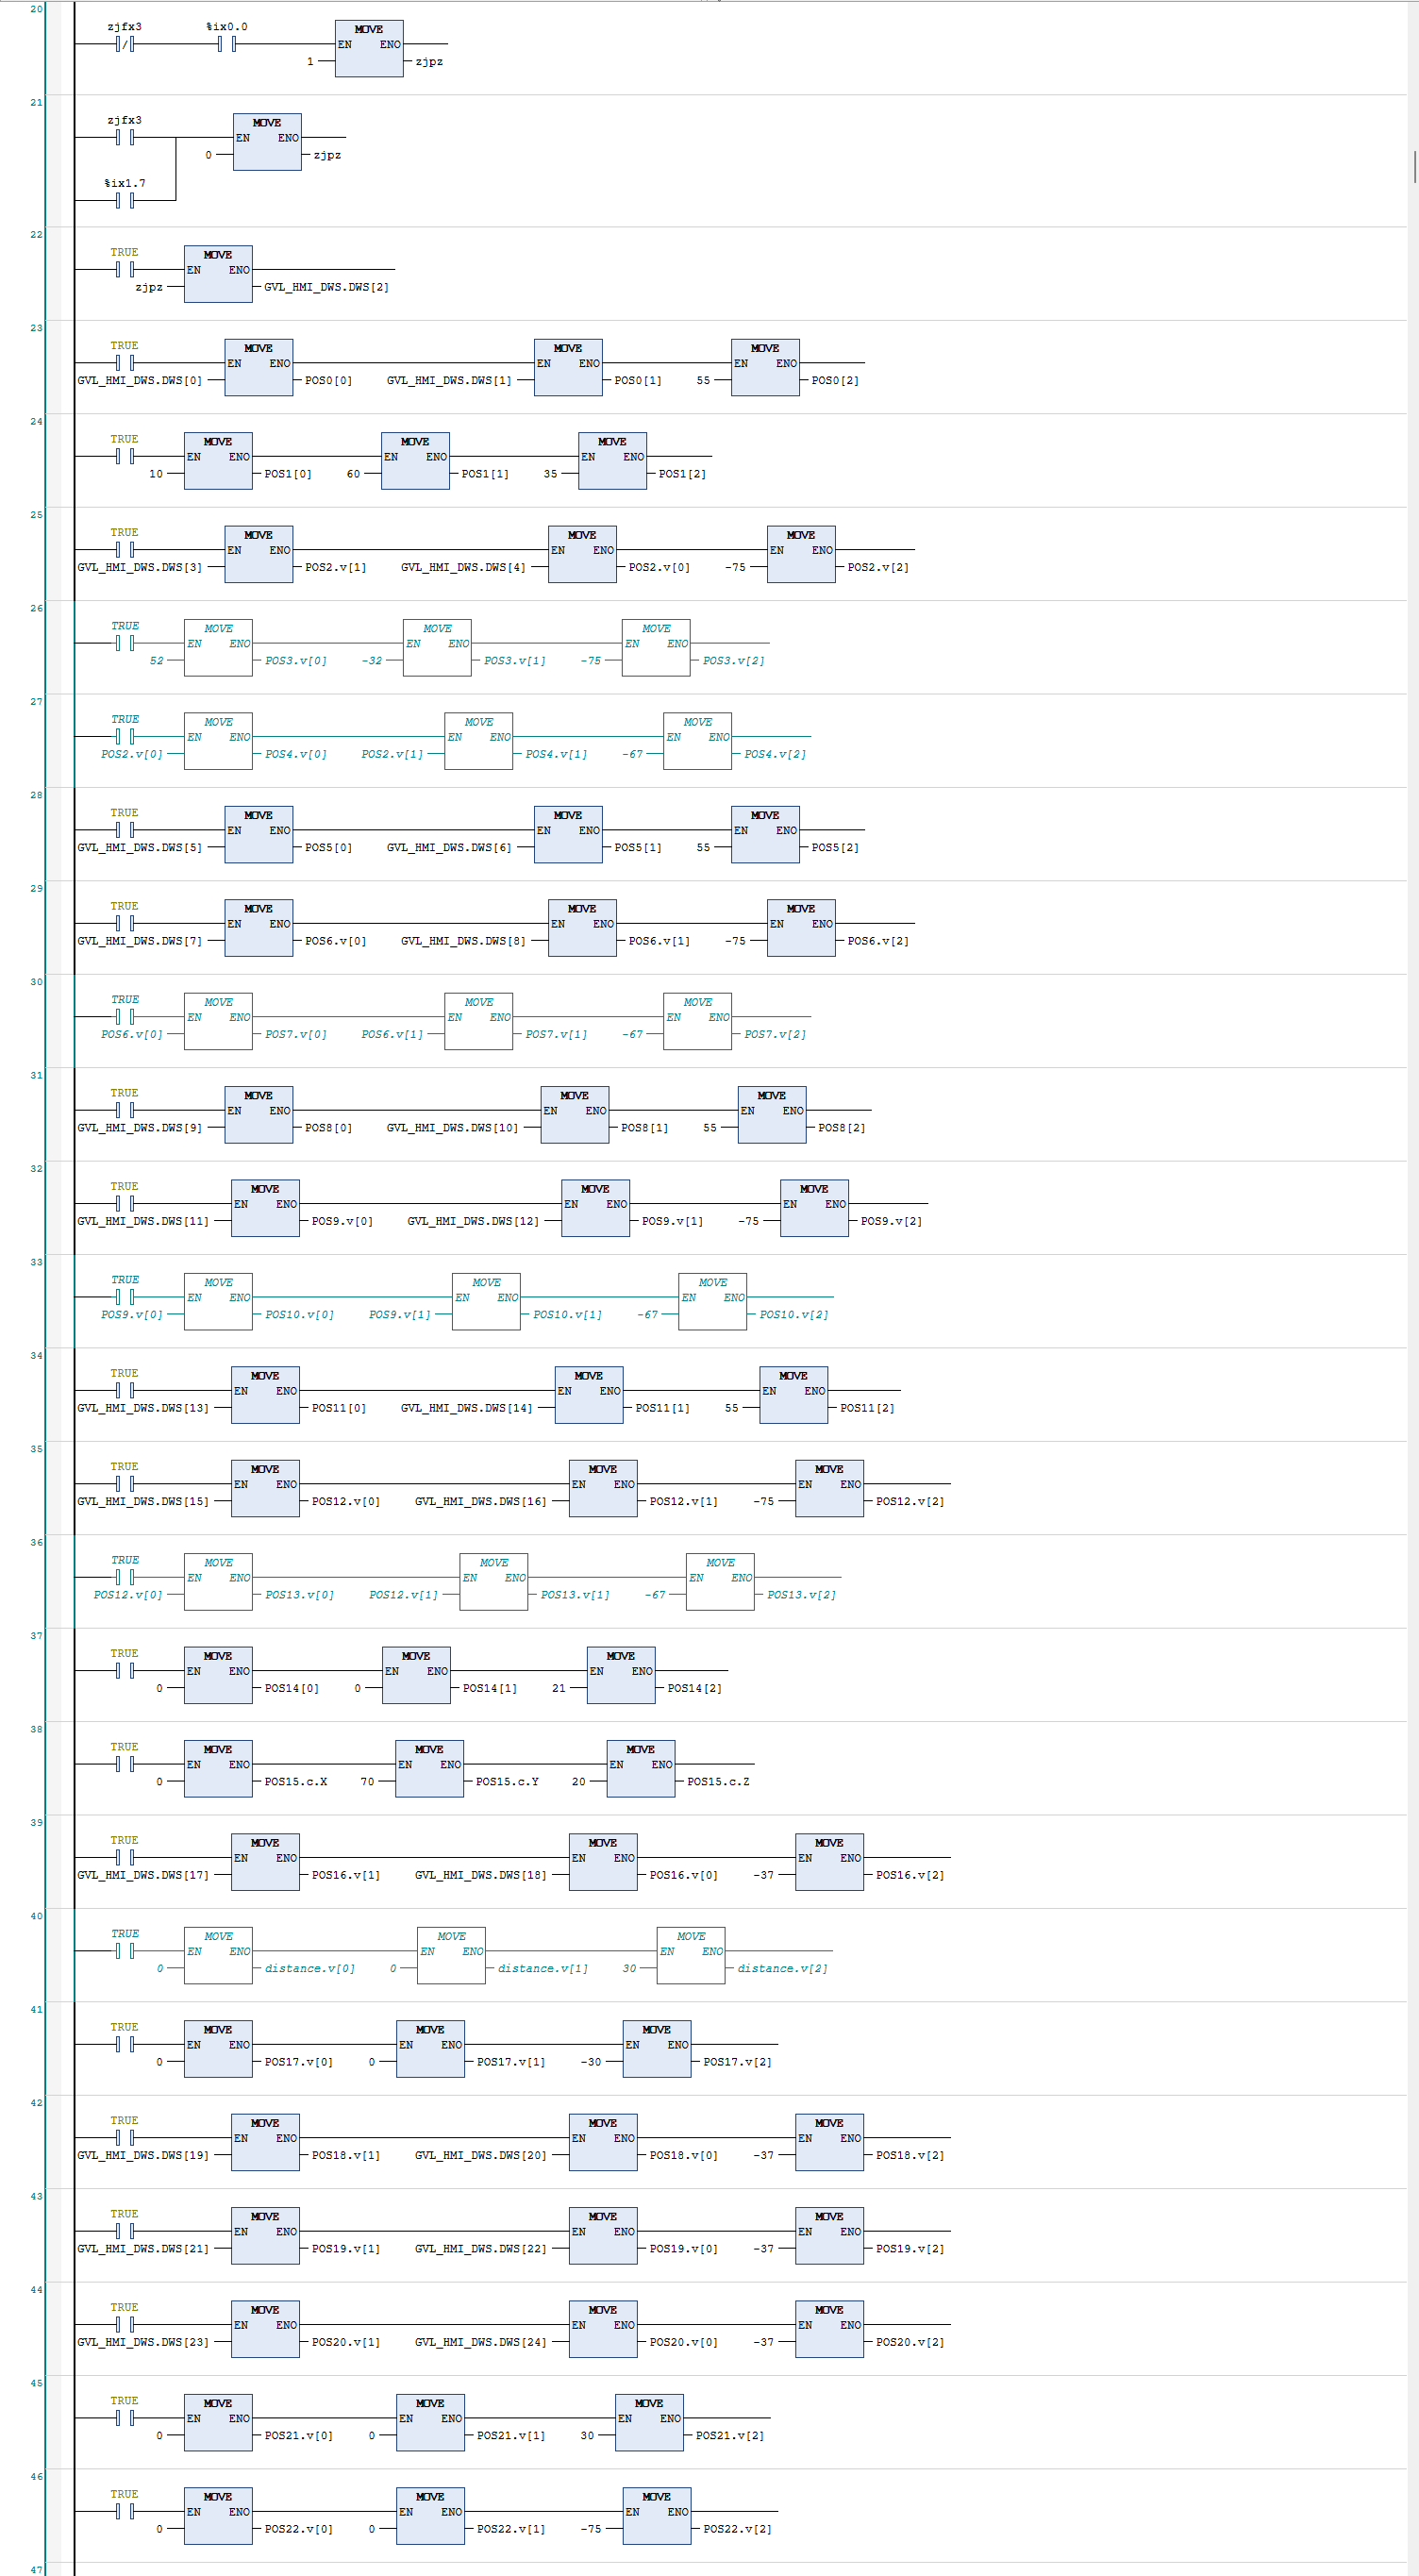
\includegraphics[width=\linewidth,height=0.42\textheight,keepaspectratio]{2与视觉软件通信.png}
		\caption{与视觉软件通信}
		\label{fig:plc-vision-comm}
	\end{subfigure}
	
	\caption{PLC程序：准备使能与视觉通信}
	\label{fig:plc-enable-vision}
\end{figure}

\begin{figure}[H]
	\centering
	
	\begin{subfigure}[t]{0.49\textwidth}
		\centering
		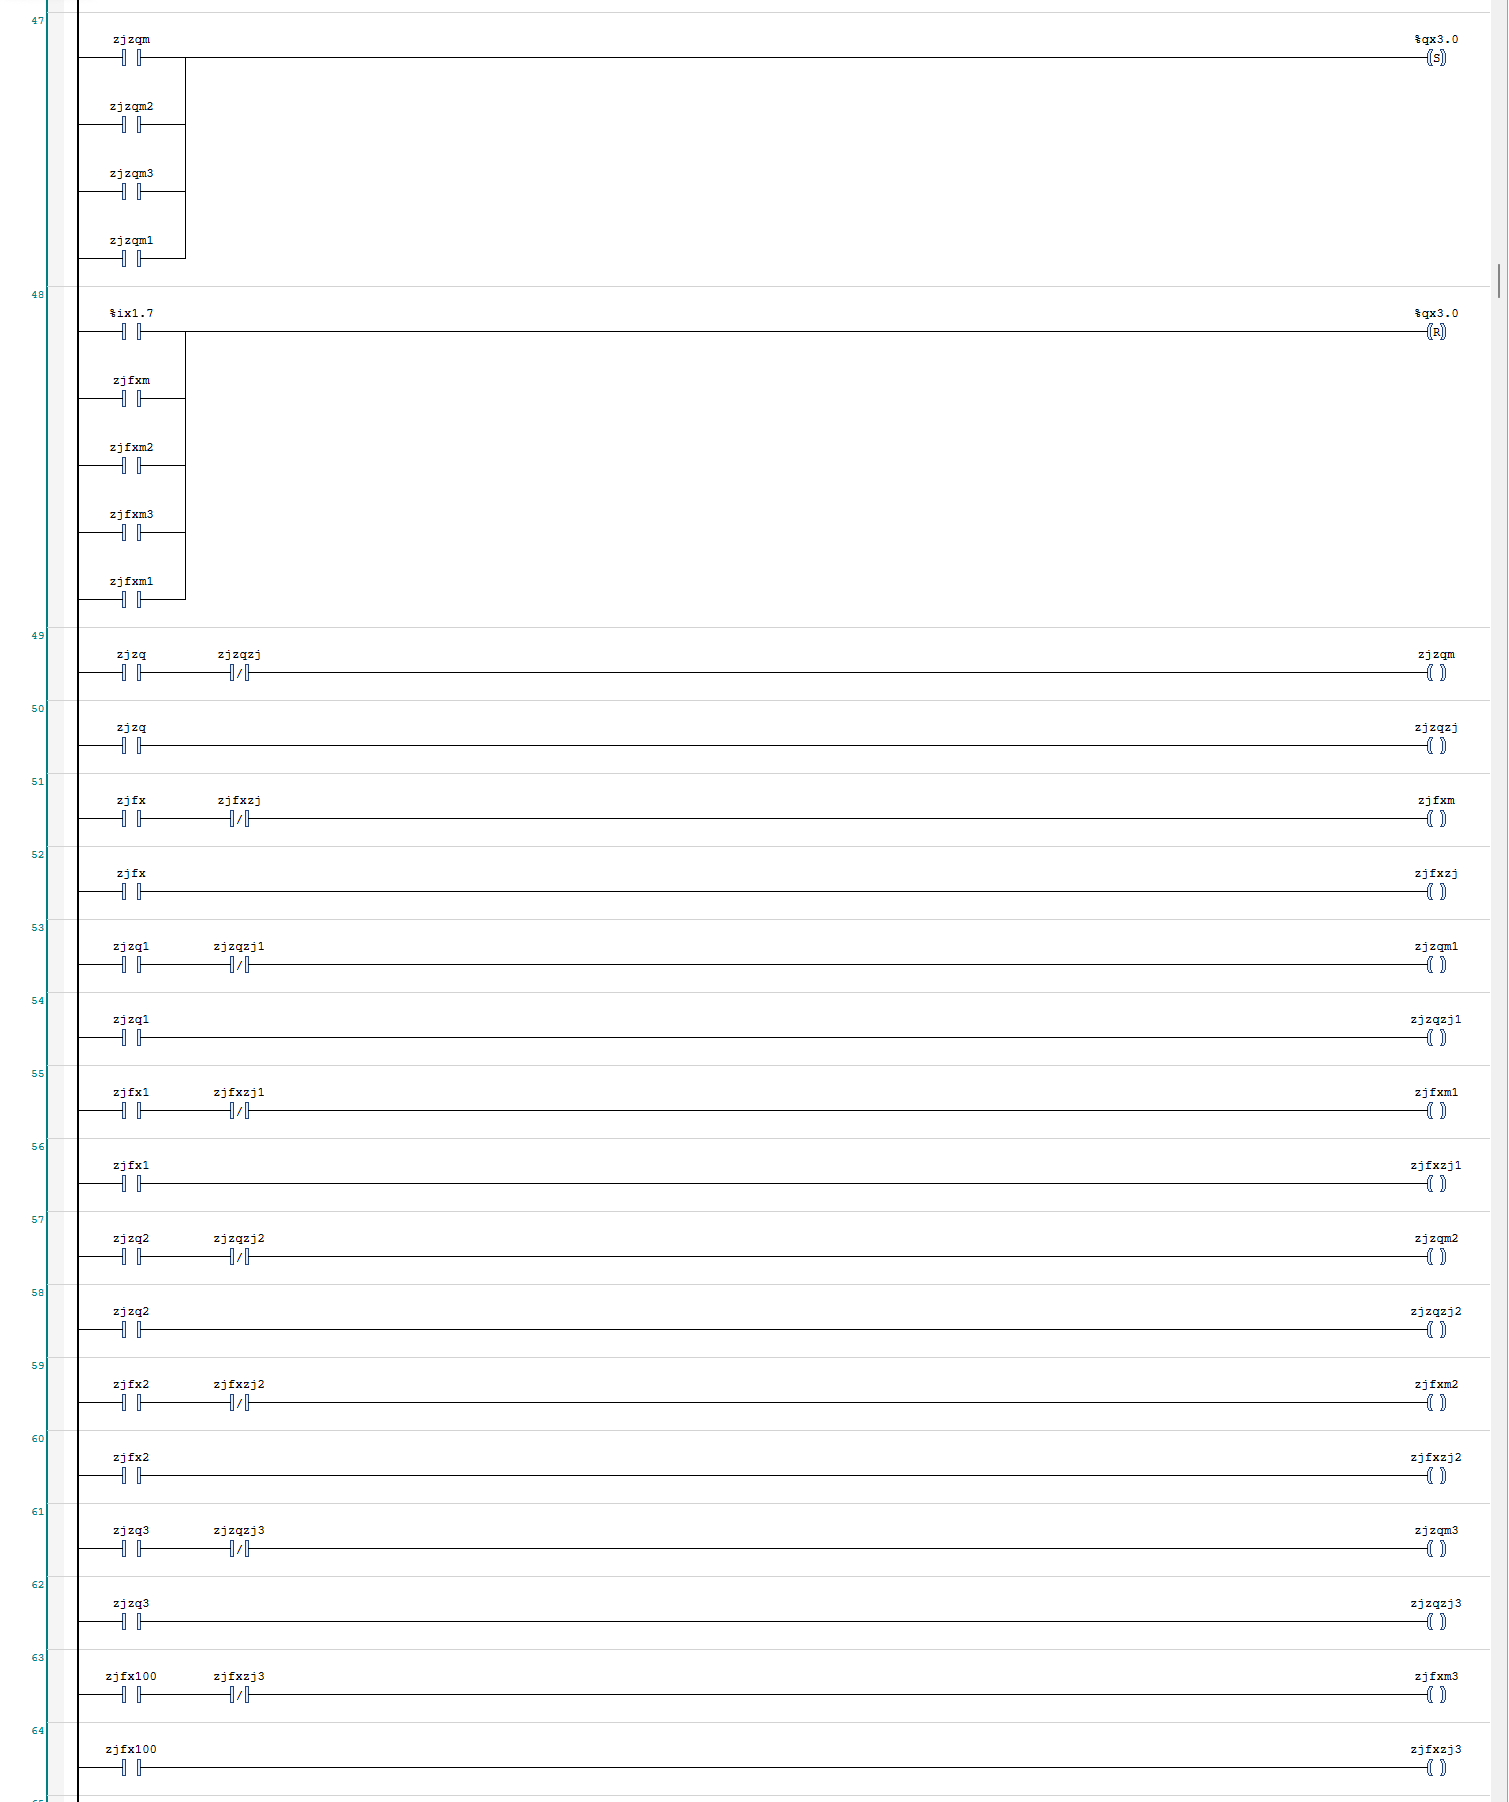
\includegraphics[width=\linewidth,height=0.42\textheight,keepaspectratio]{3直角机器人磁铁.png}
		\caption{直角机器人电磁铁控制}
		\label{fig:plc-cart-mag}
	\end{subfigure}
	\hfill
	\begin{subfigure}[t]{0.49\textwidth}
		\centering
		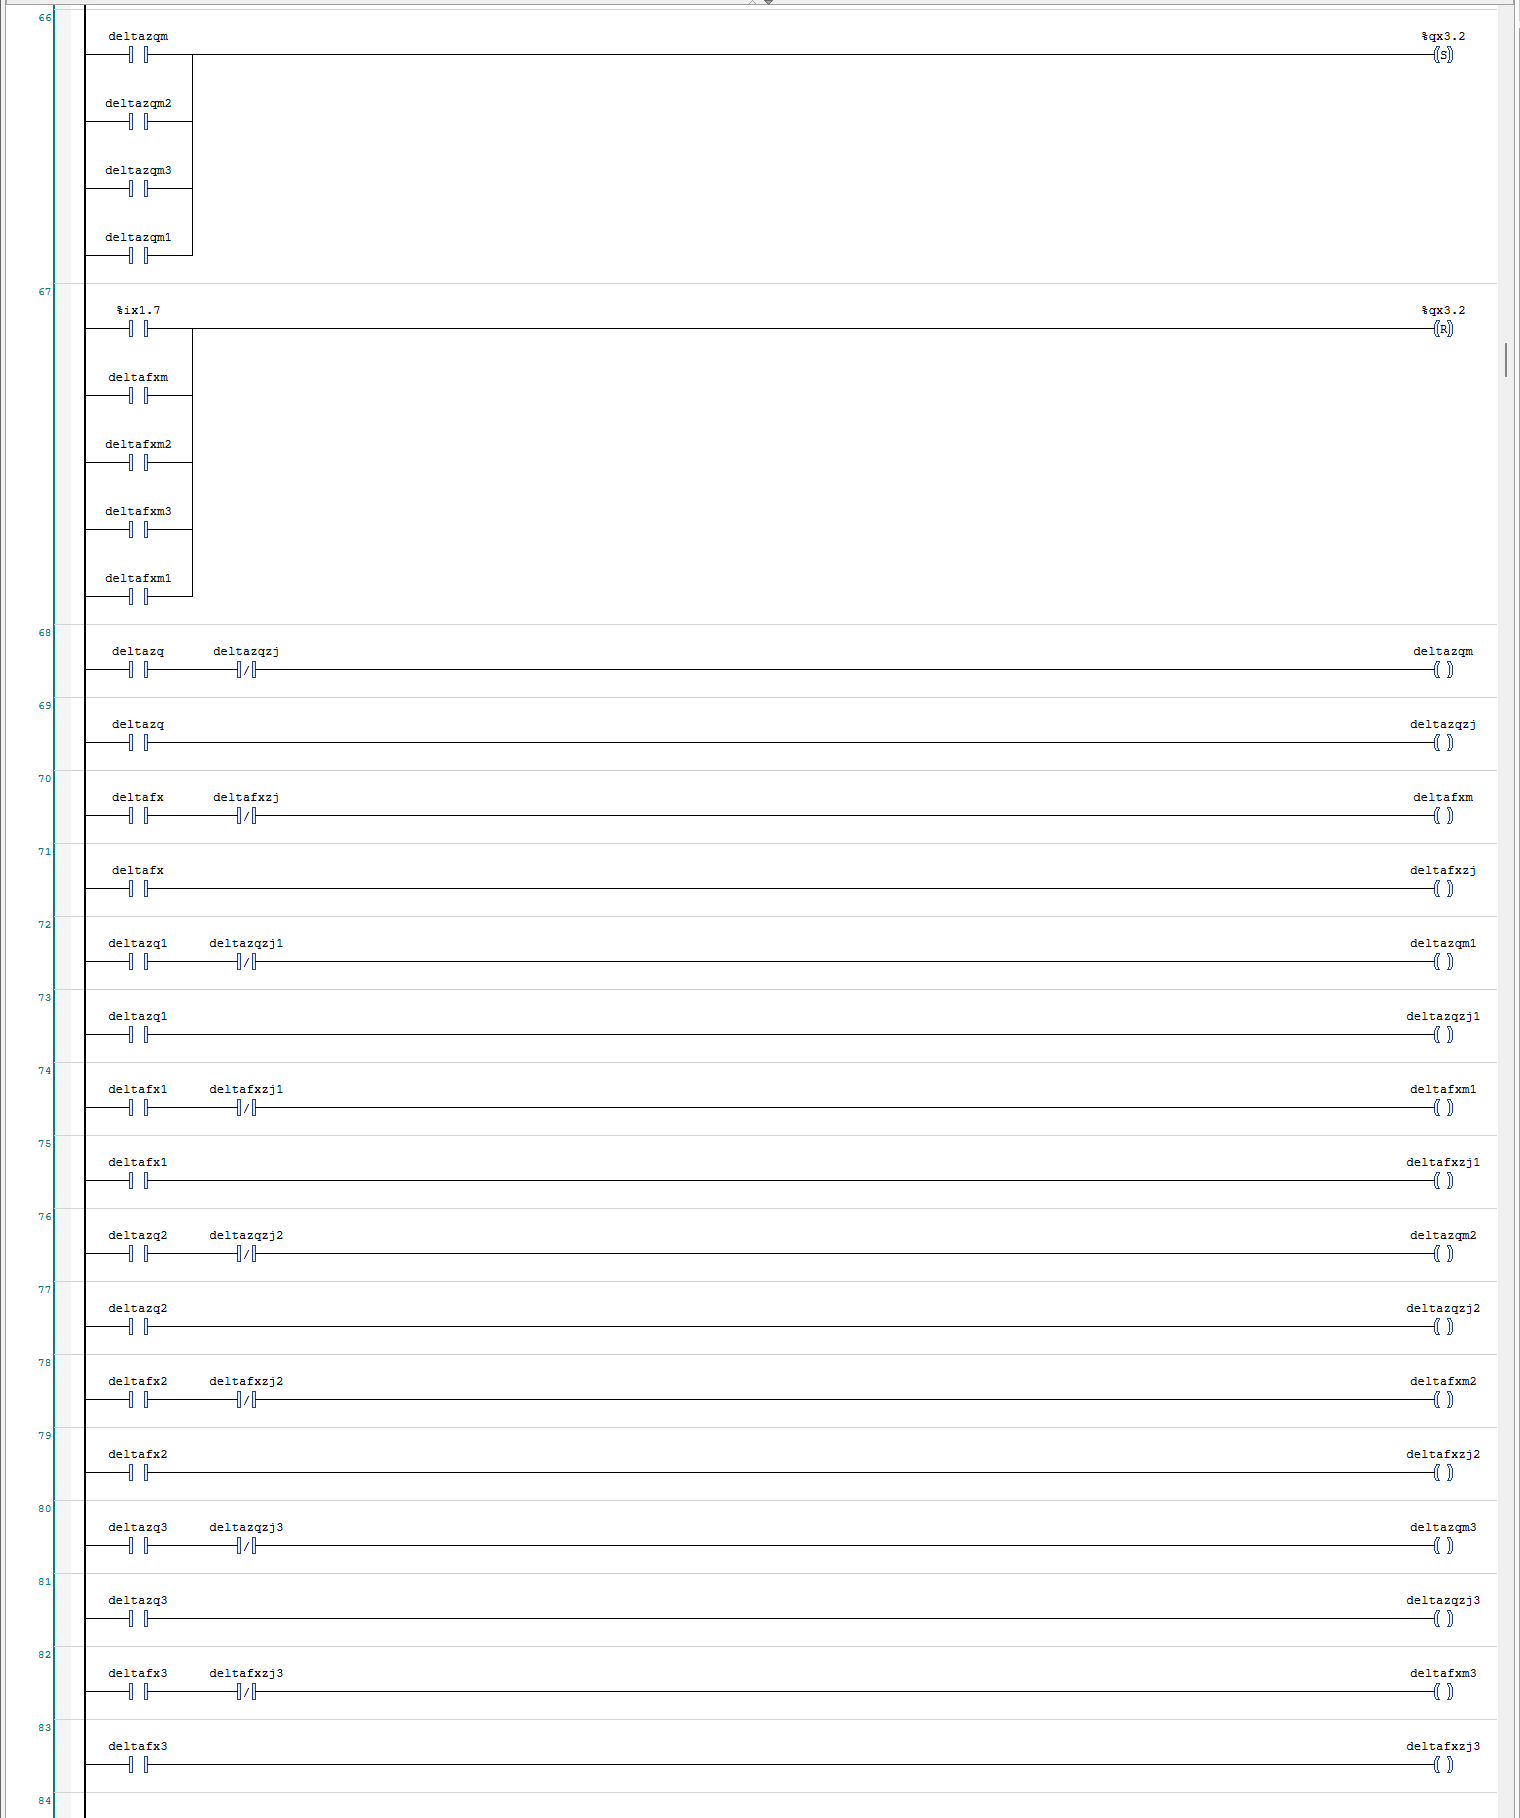
\includegraphics[width=\linewidth,height=0.42\textheight,keepaspectratio]{4delta机器人磁铁.png}
		\caption{Delta机器人电磁铁控制}
		\label{fig:plc-delta-mag}
	\end{subfigure}
	
	\caption{PLC程序：两类机器人电磁铁控制}
	\label{fig:plc-mag-control}
\end{figure}

直角坐标机器人的抓取与放下流程如图\ref{fig:plc-cart-pick}所示。程序会依次引导直角坐标机器人的末端到达物品上方、抓取并移动至托盘指定位置、下降放置物品。
直线伺服机器人移动程序如图\ref{fig:plc-servo}所示，用于完成托盘在搬运工位与分拣工位之间的传送，其到达分拣工位的信号会作为后续Delta视觉检测和分拣动作的前置条件。
Delta机器人移开拍照程序如图\ref{fig:plc-delta-move-away}所示。该动作是为了让分拣工位上的物品能够不被机器人本体或末端执行器遮挡，被Delta机器人侧的相机拍全，从而保障物品视觉识别的稳定性。
轮询使能拍照程序如图\ref{fig:plc-poll-photo}所示，用于直线伺服机器人到达分拣工位时向视觉系统发送触发信号，并且等待视觉软件完成识别后再进入下一步。
Delta机器人抓取与放下流程如图\ref{fig:plc-delta-pick}所示。它根据Delta机器人侧的视觉系统返回的物品位置进行分拣，是整个流程的最后一步。

\begin{figure}[H]
  \centering
  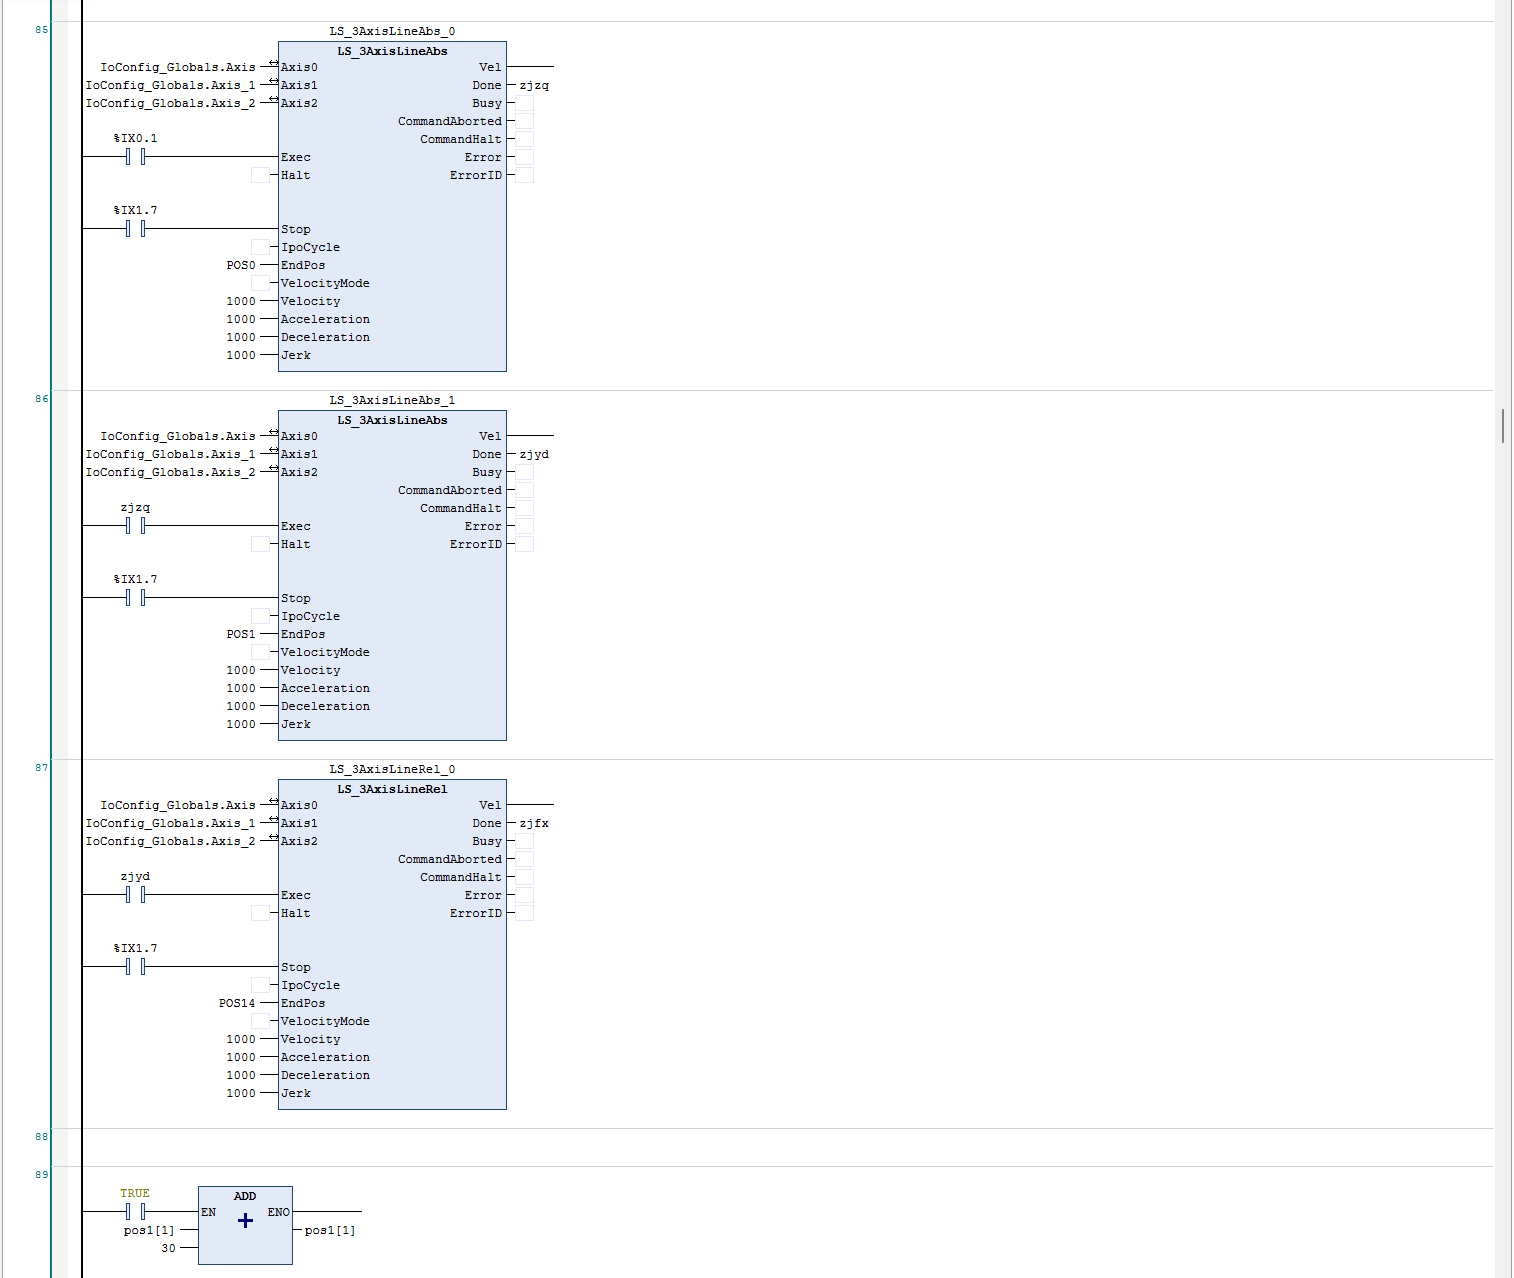
\includegraphics[width=0.96\textwidth,height=0.62\textheight,keepaspectratio]{5直角机器人抓取与放下.png}
  \caption{PLC程序：直角机器人抓取与放下}
  \label{fig:plc-cart-pick}
\end{figure}

\begin{figure}[H]
  \centering
  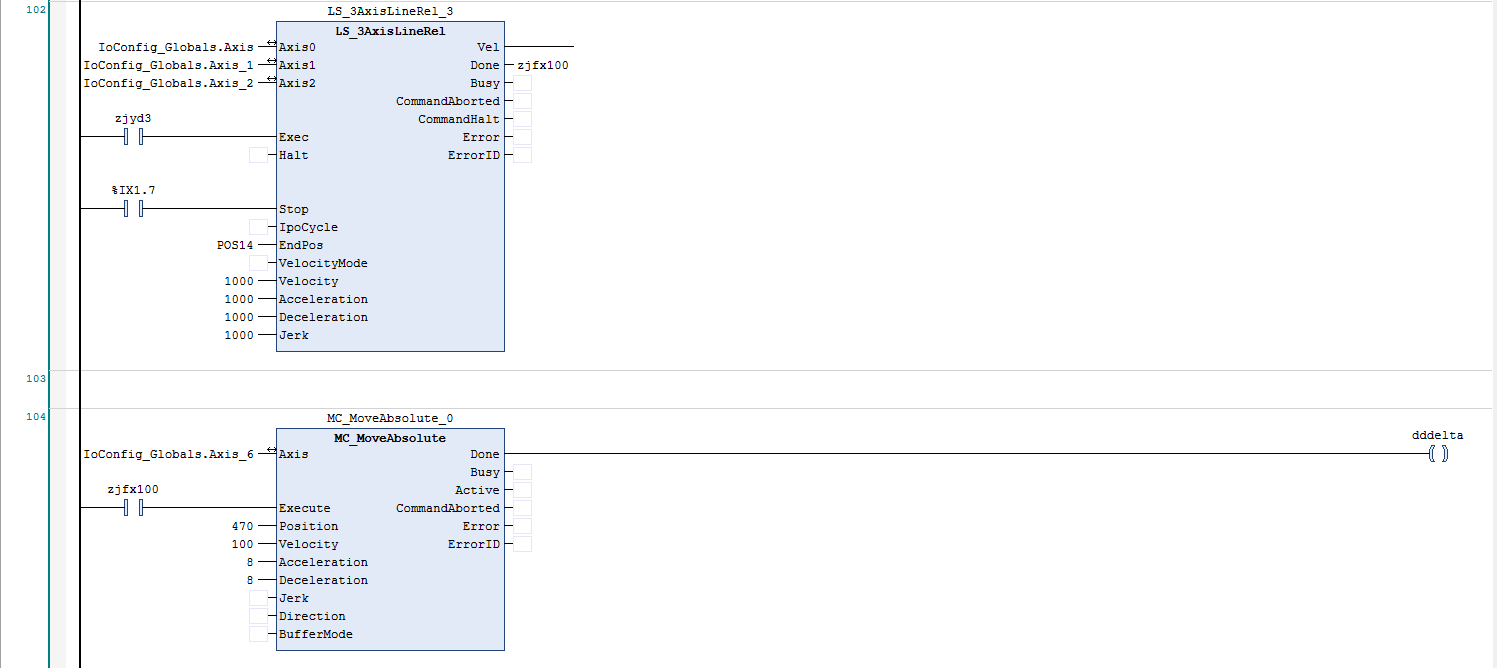
\includegraphics[width=0.96\textwidth,height=0.62\textheight,keepaspectratio]{6直线伺服机器人移动.png}
  \caption{PLC程序：直线伺服机器人移动}
  \label{fig:plc-servo}
\end{figure}

\begin{figure}[H]
  \centering
  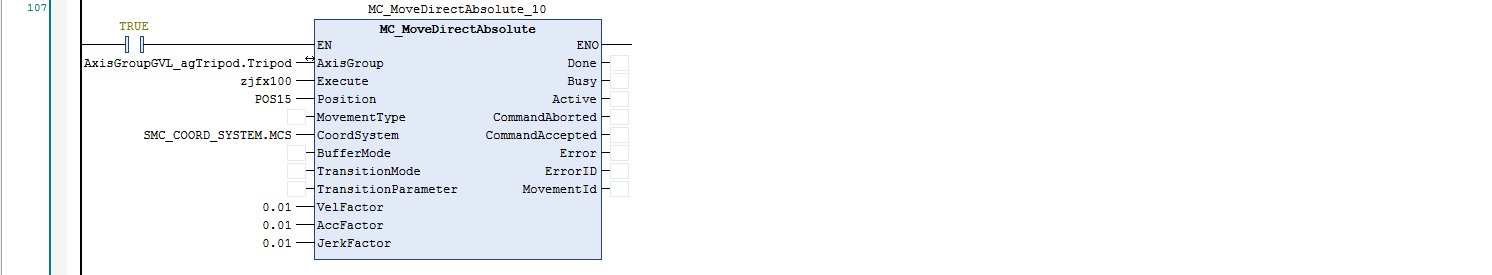
\includegraphics[width=0.96\textwidth,height=0.62\textheight,keepaspectratio]{7delta机器人移开来拍照.png}
  \caption{PLC程序：Delta机器人移开进行拍照}
  \label{fig:plc-delta-move-away}
\end{figure}

\begin{figure}[H]
  \centering
  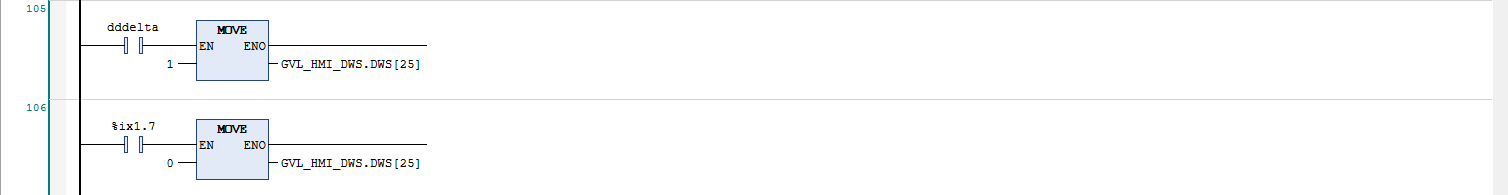
\includegraphics[width=0.96\textwidth,height=0.50\textheight,keepaspectratio]{8与视觉通信来轮询使能进行拍照.png}
  \caption{PLC程序：与视觉通信并轮询使能拍照}
  \label{fig:plc-poll-photo}
\end{figure}

\subsubsection{视觉程序流程}

视觉程序由VisionMaster软件完成配置。直角机器人视觉部分如图\ref{fig:vm-cart}所示，其主要任务是识别初始区域内物料的位置和颜色，并使用视觉软件里标定板得到的标定文件，把像素坐标转换为机器人坐标系下的坐标，并发送给PLC。

标定部分如图\ref{fig:vm-calib}所示。标定的作用是建立像素坐标与机器人坐标系之间的变化矩阵。我们在实验中注意到，在用视觉软件进行标定时，应该让直角机器人和Delta机器人都在原点沿着z轴向下移动一段距离以贴近纸面，后续再给推开，以此确保标定纸原点与机器人坐标系的原点重合，这样在后续变量计算里矫正标定时可以减少一个截距量的调整，提高调试速度。

\begin{figure}[H]
  \centering
  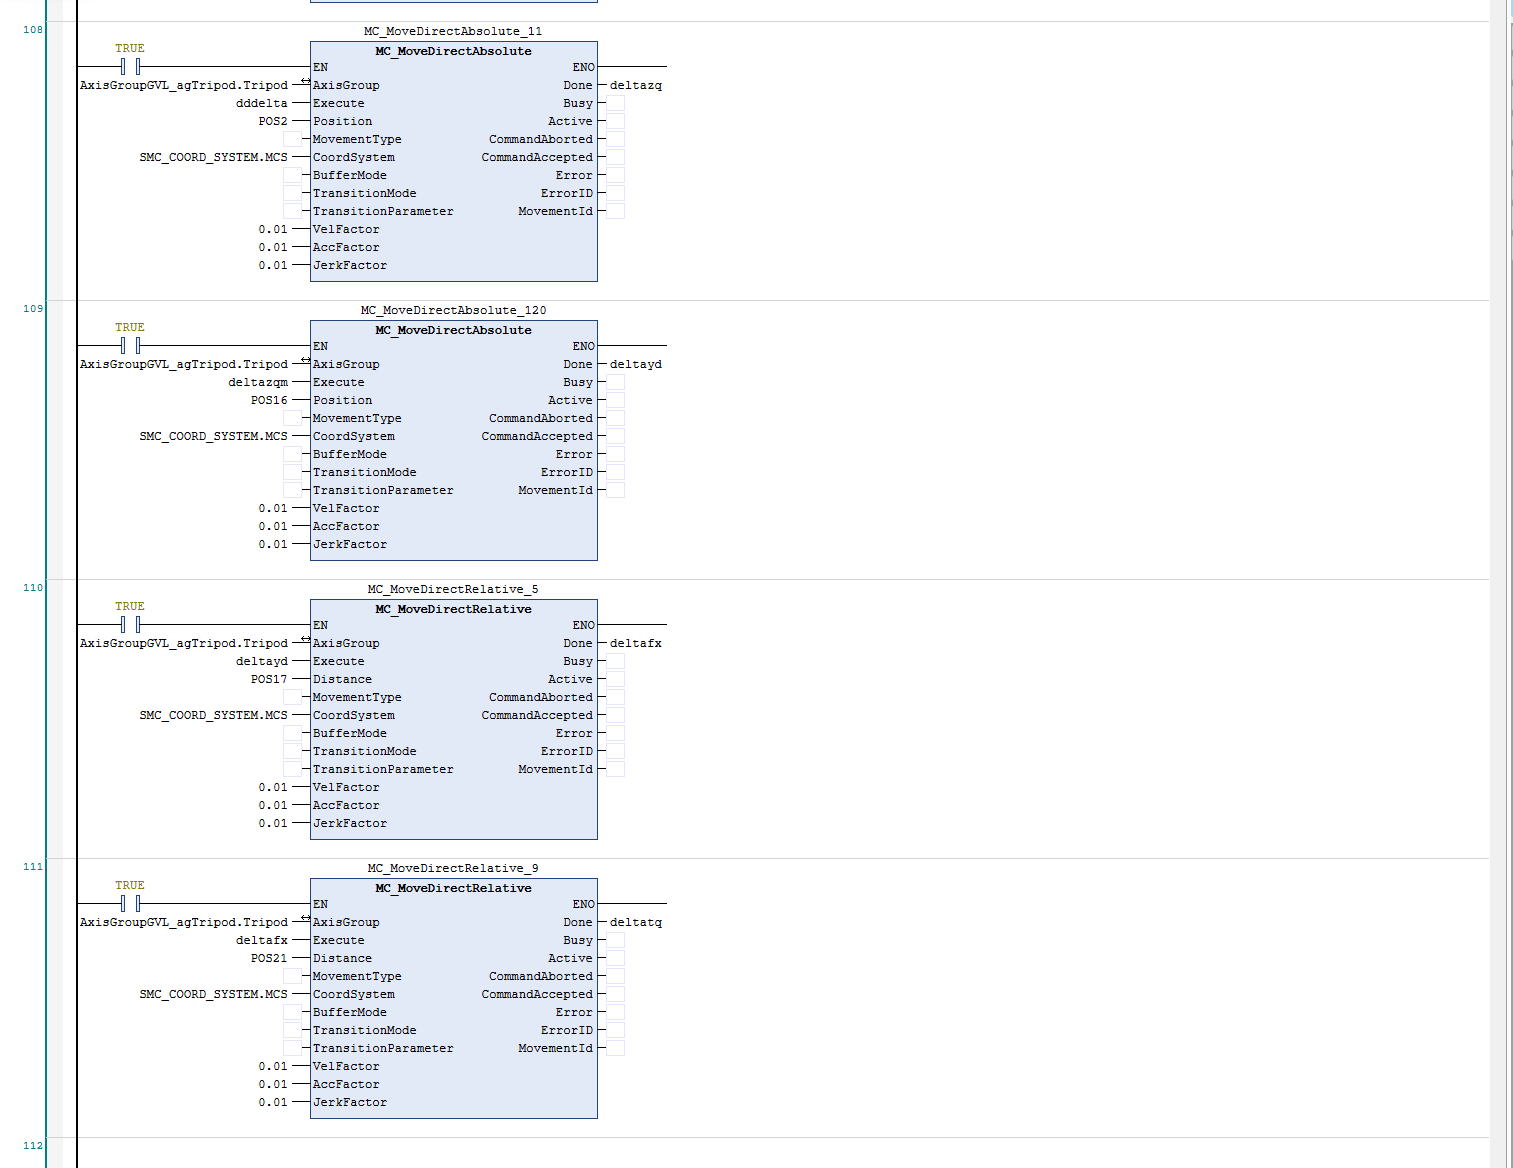
\includegraphics[width=0.96\textwidth,height=0.72\textheight,keepaspectratio]{9delta机器人抓取与放下.png}
  \caption{PLC程序：Delta机器人抓取与放下}
  \label{fig:plc-delta-pick}
\end{figure}

\begin{figure}[H]
  \centering
  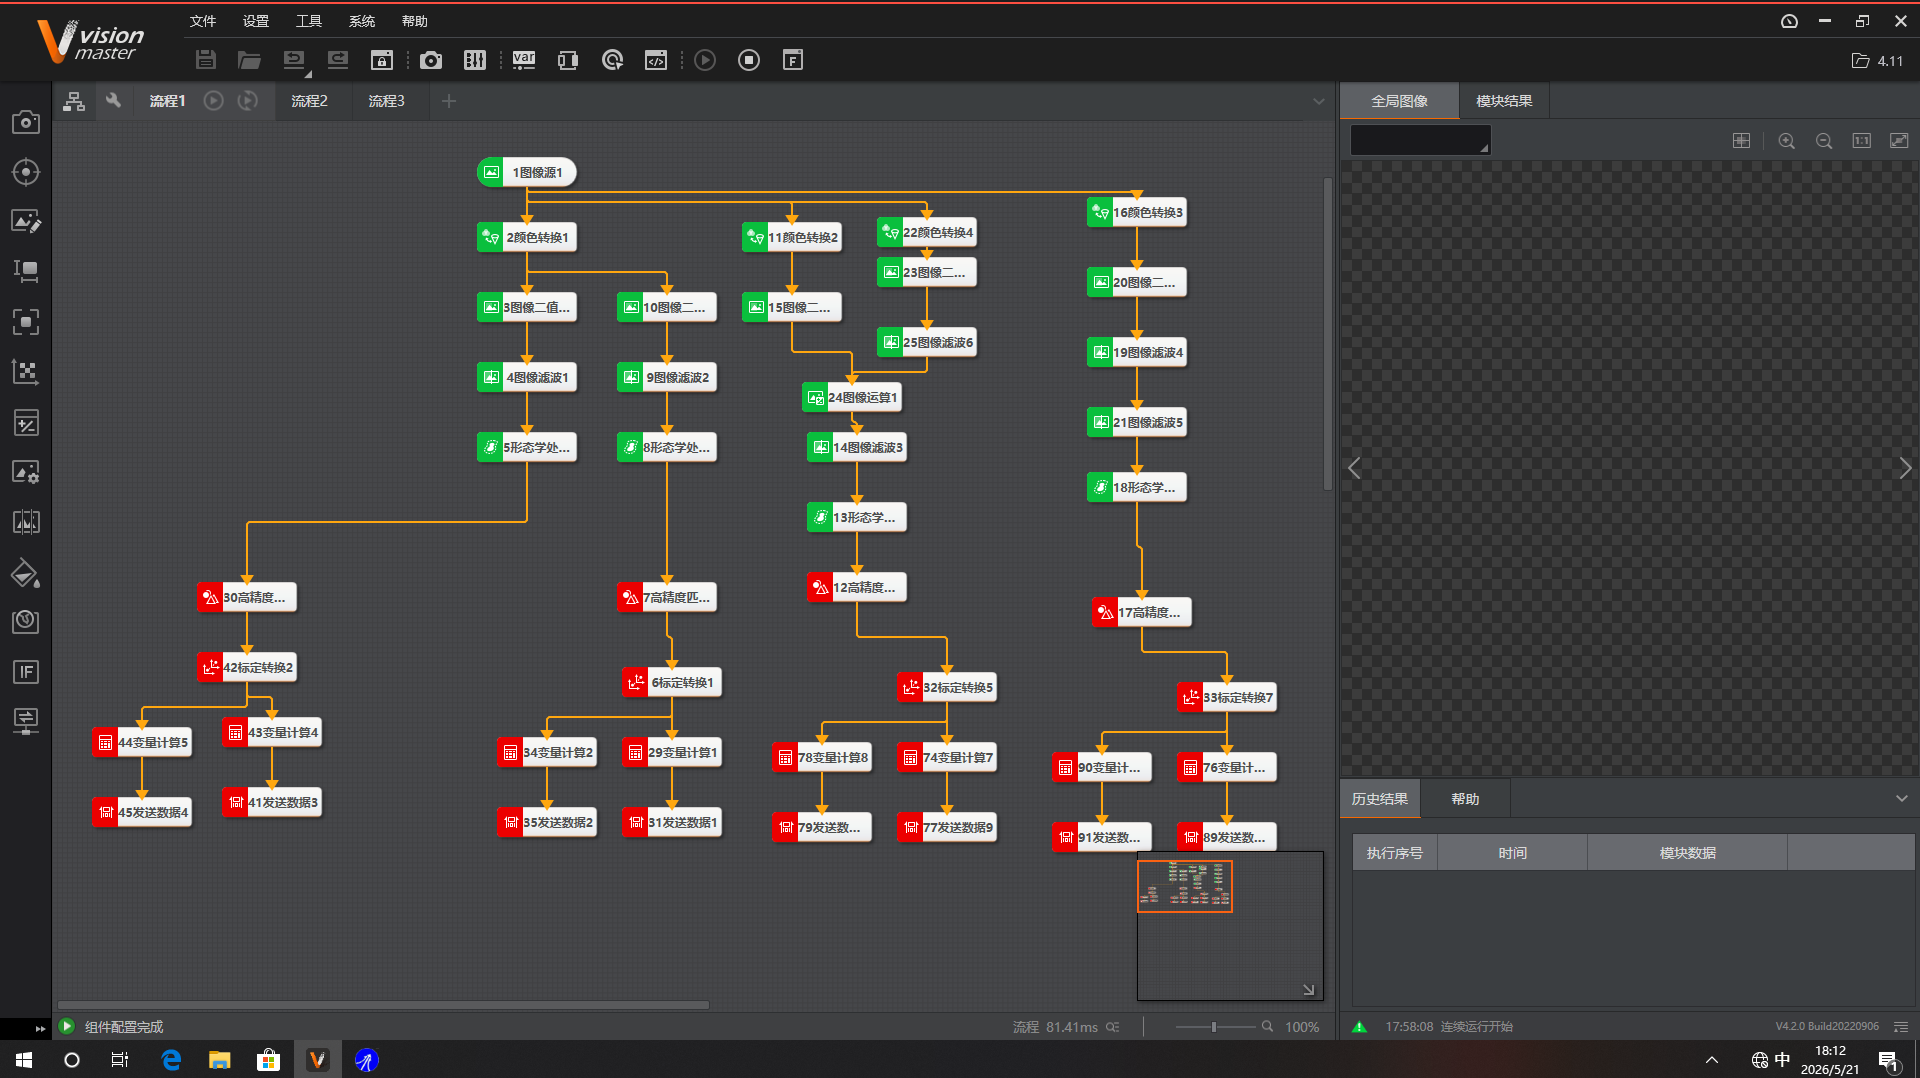
\includegraphics[width=0.96\textwidth,height=0.72\textheight,keepaspectratio]{直角机器人视觉部分.png}
  \caption{VisionMaster：直角机器人视觉部分}
  \label{fig:vm-cart}
\end{figure}

\begin{figure}[H]
  \centering
  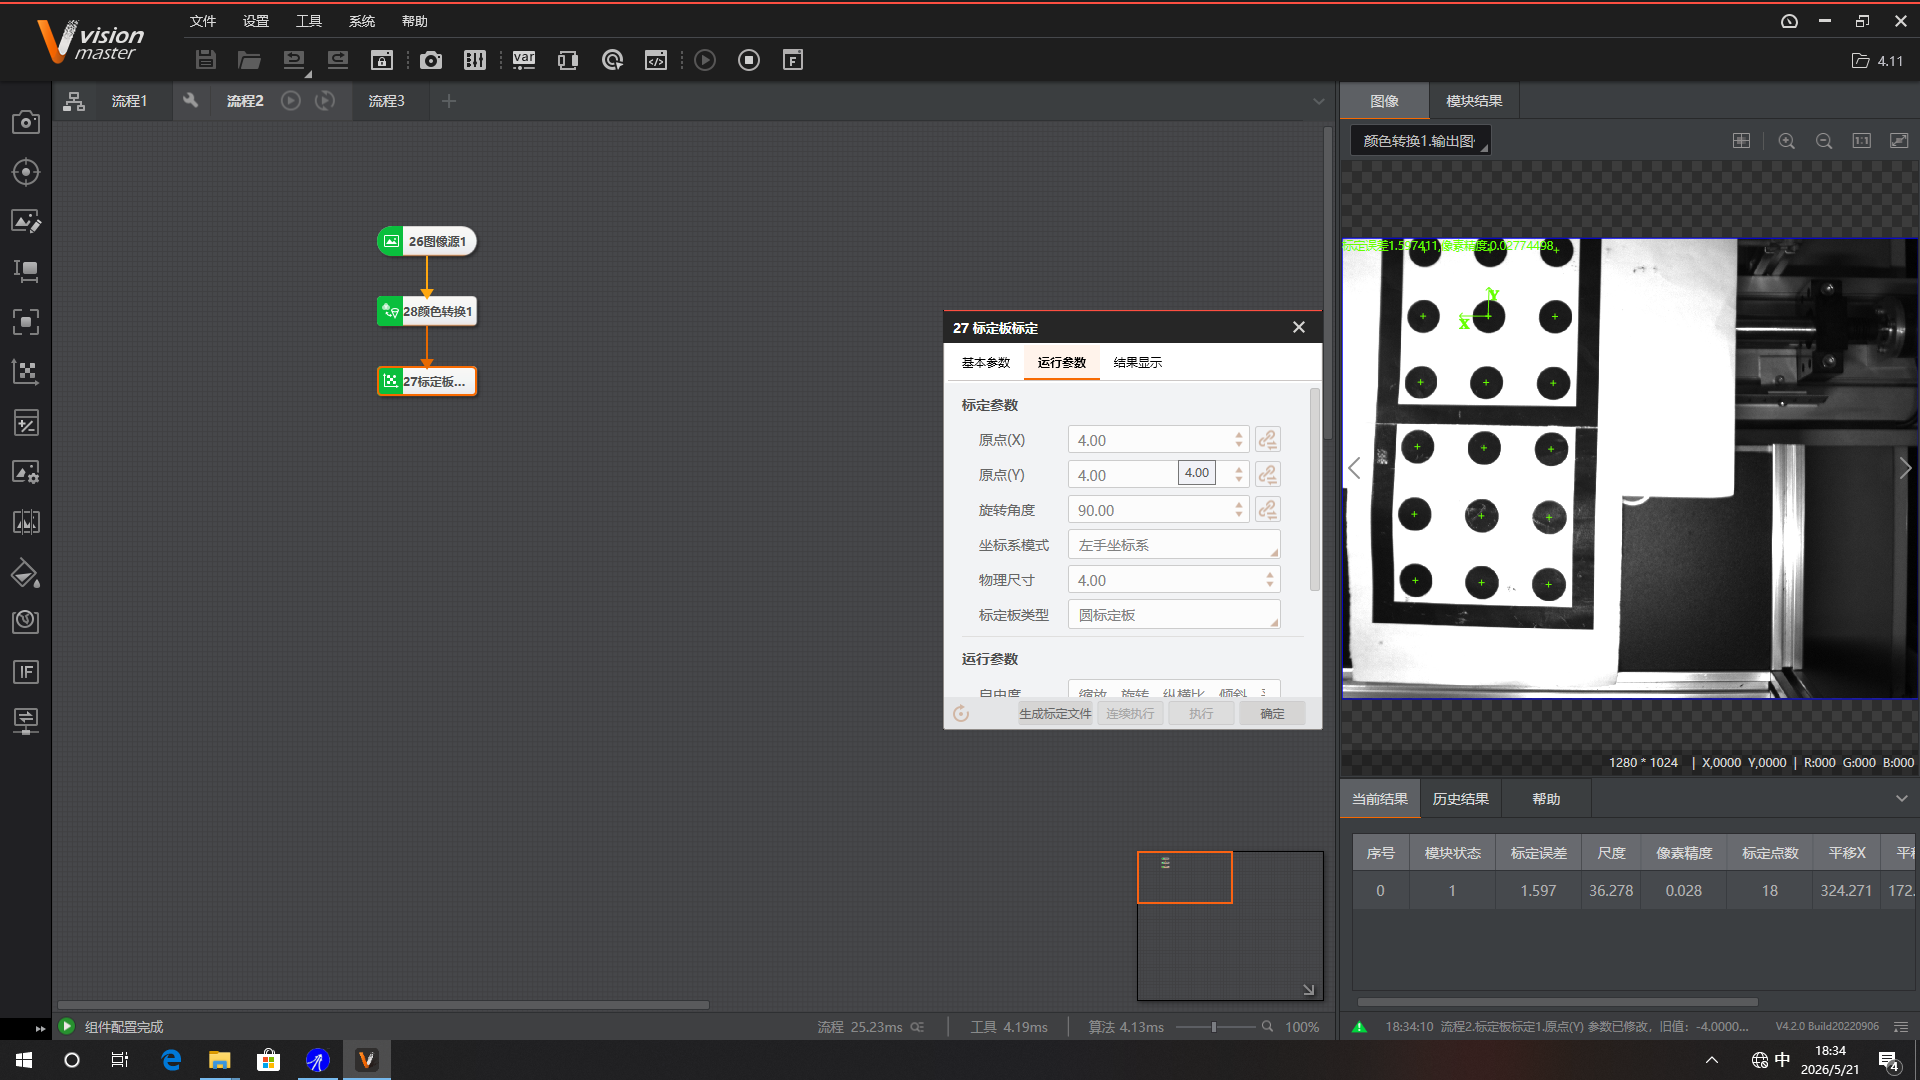
\includegraphics[width=0.96\textwidth,height=0.72\textheight,keepaspectratio]{标定部分.png}
  \caption{VisionMaster：视觉标定部分}
  \label{fig:vm-calib}
\end{figure}

\begin{figure}[H]
  \centering
  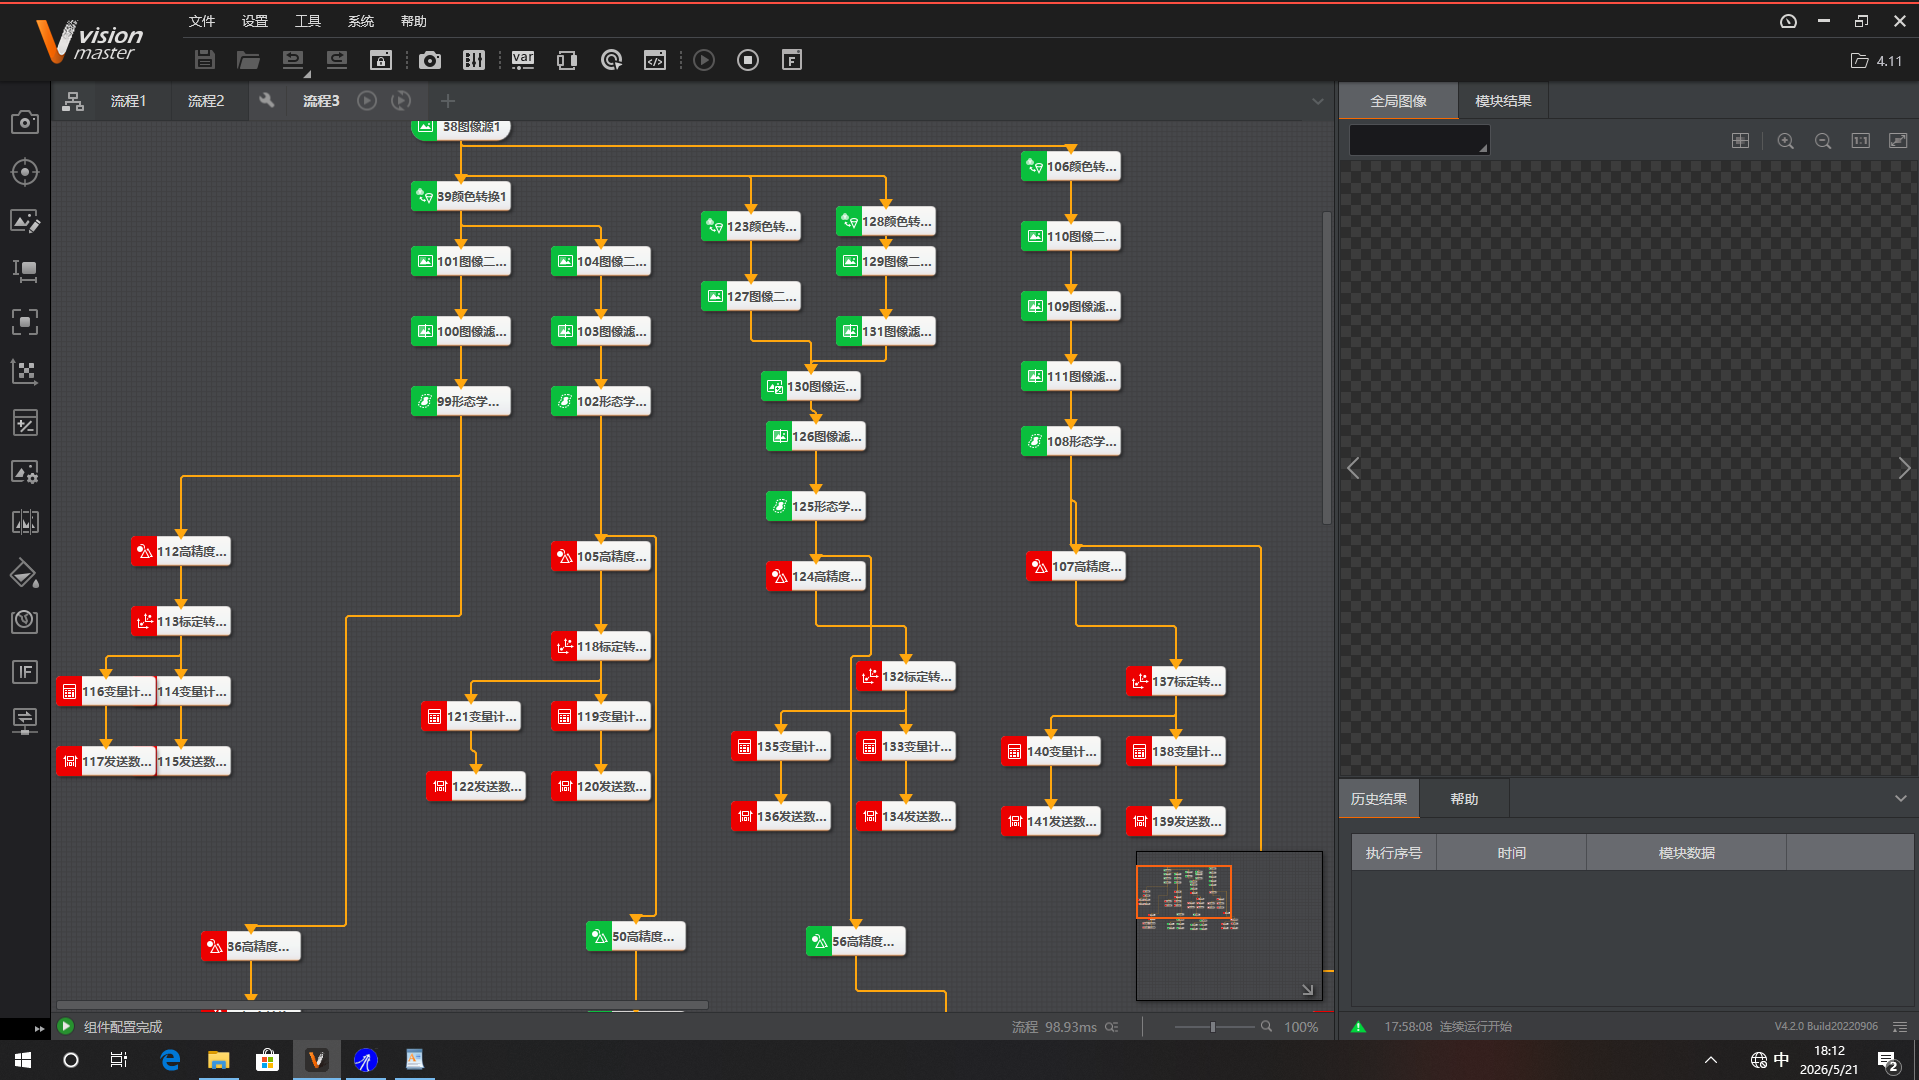
\includegraphics[width=0.96\textwidth,height=0.72\textheight,keepaspectratio]{delta机器人视觉部分.png}
  \caption{VisionMaster：Delta机器人视觉部分}
  \label{fig:vm-delta}
\end{figure}

Delta机器人视觉部分如图\ref{fig:vm-delta}所示。该流程负责识别进入分拣工位后的物品，把抓取和放下物品的位置传给PLC进而引导Delta机器人去工作。与直角机器人视觉相比，Delta侧视觉对精度要求更高，因为最终摆放的误差是直接从这里体现出来的。值得一提的是，为了避免视觉识别出的物品不停旋转，以及每次识别物体的中心不一定精准这两个问题，我们采取了三重保障措施：首先是之前提过的引入轮询使能拍照功能，这样单次拍照执行可以避免视频流里物体旋转的问题；再是在高精度匹配里选择模板数量为1，且针对圆形、三角形、正方形、五边形和圆形分别把角度定为0-120°、0-90°、0-72°以及0-1°；最后我们在高精度匹配的模板里手动点击几何中心，这样可以有效避免识别的物品中心不精准的现象。

\subsubsection{视觉与PLC通信}

视觉与PLC通信的想法是：PLC在需要拍照时置位整型的触发变量，VisionMaster在收到有效的上升沿触发事件后运行相应侧的视觉流程，并会把识别结果写入对应通信变量。PLC能够自动读取变量，指导机器人运动到指定位置。

调试初期曾使用VisionMaster的字符串触发方式，希望通过PLC发送photo\_on变量控制拍照，其中photo\_on=1表示启动视觉流程，photo\_on=0表示停止或不触发。但实际运行时出现了发送0或发送1都会触发的问题。分析后可知，字符串触发更接近于“收到某个字符串报文就触发”，它关注的是报文到达事件，而不是变量数值是否等于1。因此该方式不适宜用于判断photo\_on变量的具体数值。

后续方案改为在设备通信界面里定义一个新的接收事件：INT类型的变量photo\_on从0变成1的上升沿事件，以这个事件被触发作为作为轮询使能拍照流程开始的信号。于是视觉流程只在PLC发送有效触发条件时执行，避免了之前数值为0时仍然启动流程的问题。

\section{安装调试}

\subsection{安装调试过程}

系统调试首先从对所有机器人电机进行单独动作测试（MC\_Jog）开始，确认各轴使能、复位、脉冲指令数、点动和定位动作正常；然后对两套电磁铁进行通电断电测试，确认没有出现磁铁高温消磁的现象。之后再开展视觉系统调试，手动检查相机画面、识别流程设置、为避免镜头焦段和对焦被修改重新做视觉标定，然后检查视觉侧发送的数据与PLC接受的数据的一致性。

在单机动作基本稳定后，系统进入分段联调。第一阶段验证直角机器人侧视觉检测和抓取动作，即视觉识别初始物料后，PLC能否根据坐标驱动直角坐标机器人完成吸附和放置。第二阶段验证伺服直线模组的托盘传送，使物料能够从前端搬运区到达Delta分拣区。第三阶段验证Delta侧视觉检测和分拣动作，确认机器人移开拍照、视觉识别、坐标读取、抓取和目标位置放置能够连续执行。最后再进行全流程自动运行测试，使启动、复位、视觉触发、机器人动作和分拣结果形成闭环。

\subsection{故障分析}

调试中遇到的第一个问题是PLC软件有时无法正常写入程序，甚至出现PLC上的程序反过来把电脑端文件覆写掉的情况，常常发生在软件连续运行较长时间时，处理方法是关闭并重启PLC编程软件，重新登录控制器后再进行程序的下载。经过该方式处理后，工程写入可以恢复正常。

第二个问题是Delta机器人工作空间边缘误差较大。调试中发现，Delta机器人中心区域定位较准，但越靠近边缘误差越明显；即使在同一侧区域内移动较小距离，所需补偿量也会变化。最初尝试把三张标定贴在一起，确保每个点之间的距离都是标准的4 cm，并借助标定纸圆点测量6个点的机器人坐标和像素坐标，求取二维仿射矩阵$T^{Delta}_{pixel}$，见\eqref{biaoding}。该方法能够表达线性的变换关系，但实际中并未通过该方法稳定提升抓取精度，说明误差不是能靠线性的校正解决的。

\subsection{误差分析}

Delta机器人边缘误差的主要缘由在于并联机构工作空间边缘存在非线性误差，而二维仿射矩阵只能处理线性平移、旋转、比例和剪切，无法充分修正边缘区域的非线性变化。在反复的实测中我们发现，误差与物品颜色形状无关，只与物品摆放的位置相关，具体来说，较大的误差出现在Delta机器人$x<0$的一侧，且主要体现为$y$方向偏差；另外这个偏差与$|x|$近似成正比。因此最终采用经验补偿：
\[
y_{corr}=y+0.005x
\]
其中$x$为Delta机器人坐标中的x坐标，$y_{corr}$为补偿后的机器人目标点位的y坐标。

除坐标补偿外，最终放置阶段还额外降低了Delta机器人的速度和加速度。实验发现，这一步可以显著减少末端高速运动后释放物品时产生的偏移，进而大幅降低放置误差。经过坐标补偿和运动参数调整这套组合拳后，Delta侧的摆放误差由约4 mm降低到2 mm左右，基本满足精度要求。

从误差来源看，本系统的误差主要包括视觉识别误差、标定误差、机构定位误差、末端吸附和释放误差。实际调试表明，误差改进不能只依赖单一软件补偿，而需要把视觉、机械和运动参数结合起来处理。

\section{总结与收获}

本项目完成了直角坐标机器人搬运、伺服直线模组传送、Delta机器人分拣以及双视觉识别的系统集成。PLC程序按照运行流程完成了轴使能复位、视觉触发、数据通信、机器人运动、电磁铁控制和动作互锁，使无序物品能够按照视觉检测结果完成自动搬运和分类摆放。VisionMaster视觉流程分别承担初始区域和目标区域检测任务，为机器人提供位置和类别信息。通过分阶段调试，系统从单机构动作逐步过渡到全流程联动运行。

系统仍存在不足。首先，Delta机器人工作空间边缘的非线性误差没有从完整运动学模型层面进行补偿，目前采用的是基于测试结果的经验修正，前者是更系统更鲁棒的精度提高方法，应该尝试该方法。其次，视觉标定点数量和覆盖范围仍有提高空间，如果物料出现范围进一步扩大，现有标定结果可能会出现更大的偏差。再次，系统自动运行节拍还有尚未优化，例如部分等待时间可以在保证稳定性的基础上进一步缩短，不少机器人动作可以并行进行提高效率。

通过本次实验，我更加清楚工业机器人系统并不是孤立的编写一段机器人运动程序，而是要整体看待机构、传感、控制和通信等等组分。直角坐标机器人侧的坐标关系较为直观，但仍需要处理视觉坐标转换和抓取高度问题；Delta机器人动作速度较快，但边缘误差和末端释放稳定性对最终结果影响明显。在PLC程序设计方面，我重新认识到状态顺序和互锁条件的重要性。机器人动作不能只依靠目标位置命令，还需要结合使能状态、复位状态、运动完成信号、视觉完成信号和安全条件共同判断。

后续改进建议主要包括三点。第一，可以增加标定点数量，并使标定点覆盖整个有效工作区域，从而提高视觉坐标转换的稳定性。第二，可以针对Delta机器人建立更精细的误差补偿表或分区补偿模型，使分拣区域精度进一步提高。第三，可以对PLC程序状态进行更清晰的模块化整理，把视觉通信、运动控制和故障处理分别封装，提升程序后续维护和扩展的便利性。

\section{参考文献}

\begin{thebibliography}{99}
  \bibitem{pmc-motion} 雷赛智能控制股份有限公司. PMC600中型PLC用户手册4---运动指令篇.
  \bibitem{pmc-software} 雷赛智能控制股份有限公司. PMC600中型PLC用户手册2---软件篇.
  \bibitem{l7ec} 雷赛智能控制股份有限公司. L7EC系列用户手册V2.0.
  \bibitem{leadstudio} 雷赛智能控制股份有限公司. LeadSys Studio编程及应用手册.
  \bibitem{visionmaster} 海康机器人. VisionMaster视觉软件相关资料.
\end{thebibliography}

\end{document}
